\documentclass[11pt,twocolumn]{article}

\usepackage{graphicx}
\usepackage{setspace}
\usepackage{url}
\usepackage[left=1in,top=1in,right=1in,bottom=1in,nohead]{geometry}

\author{Kyle Conroy and Brandon Liu\\
http://www.github.com/derferman/bitewise}
\title{Do Ethnic Neighborhoods have Better Ethnic Food?}

\begin{document}
\maketitle

\section{Introduction}

Like many great ideas, our research topic came to us over lunch. Many San Francisco residents spend their lunch hour waiting in line in front of a food truck on the city streets. With the rise in popularity of these food trucks, we are interested in their history and success. Sadly, after looking into Data SF, the official data clearinghouse for the city and country of San Francisco, food truck data is in short support, with nothing beyond the location of such trucks \cite{foodtrucks}.

Our investigation of food trucks sparked and inquiry into ethnic restaurants, particularly Mexican restaurants. We are curious about the relationship between the location and Yelp rating of a given burrito place. For example, are burrito places rated higher in the Mission than other neighborhoods? If so, than ethnic neighborhoods may tend to attract customers interested in finding quality cuisine of that ethnicity.

\section{Data ETL}

To answer this question, we use four different data sets. First, we use census data from the Federal Governmen \cite{census} to calculate demographic information about San Francisco and its surrounding areas. The United States census splits neighborhoods up into smaller plots of land named tracts. A tract is the right size for our project; in major cities, a tract spans just a few blocks. The City of San Francisco provides additional per-tract ethnicity information\cite{bcensus}, allowing us to build an accurate ethnic representation of the entire city with decent resolution. This set is stored as a CSV with the tract, the ethnicity data, and the coordinate for the tract.

Combining these two datasets involved strange data formats not popular in today's world of web APIs. Census data comes in two flavors: plain-text ASCII format or a binary format called a shape file. We found that the ASCII format was too cumbersome to use, so we went with the binary format. The open-source Python Shapefile Library \cite{shapely} made parsing the census data quick and simple. Each entry in the shape file contains data about the entry and the latitude and longitude coordinates which define its shape. These points are used to construct a polygon representing the tract. The data associated with a shape entry contains useful information such as tract number and county number. We use this data to filter out those tracts which aren't in the San Francisco area.

Our other data sets come from Yelp. Since we're investigating business ratings, Yelp is the best place to go. Yelp provides a REST API for their data with the only requirement signing up for a developer key. Using the API \cite{yelpapi}, we collected business listings for six different categories of restaurant. These categories include Mexican, Chinese, and vegetarian. Our final restaurant data set includes over 1,000 restaurants in the San Francisco area. Almost half of those restaurants fall into the Mexican category.

Yelp returned the data back in JSON, making this data much easier to process than the census data. However, Yelp limits business results to twenty per request, so we had to combine multiple responses into one large list for each restaurant type. Yelp provided more information per business then we could analyze. Their location information proved to be especially useful, as it also includes a list of neighborhoods near each business.

Yelp returned the data in great shape, but there were a few missing pieces of information we had to collect ourselves. The Yelp API provides an image link for the rating of a business instead of an float value. Our data cleaning process involved converting these links into integers for further data processing. Many of the questions we wanted to ask revolved around the cost of a meal at each restaurant. However, Yelp doesn't included this data in their API results. To get the data, we scraped each individual business page on Yelp, parsed the HTML, performed a simple search over the page for the price, and updated our saved API results. Sadly, not all businesses have a price rating, so our data set remains incomplete in this area.

Our hypothesis requires placing businesses in their correct census tract. Geospactial queries can be time-consuming when using brute-force algorithms. To query over our census data, we use the Shapely python wrapper \cite{shapely} for GEOS \cite{geos}, a popular open-source geometry engine. With these two tools, we quickly and efficiently found the census tract for each business.

\section{Experiment 1: Comparison of Means}

The very first task perfomed to investigate our hypothesis was on three major ethnic neighborhoods in San Francisco: the Mission District, Chinatown, and Japantown. We  found the mean rating of all Chinese/Japanese/Mexican restaurants inside and outside their respective district, and compared using a Student's T-Test.


\begin{center}
  \begin{tabular}{| l | c | c | c | r | }
    \hline
    Neighborhood & In & Out & n & p \\ \hline
    M/Mission & 5.81 & 4.98 & 303 & 1.8e-7 \\ \hline \hline
    C/Chinatown & 4.67 & 4.23 & 416 & 0.062 \\ \hline
    J/Japantown & 4.67 & 4.84 & 260 & 0.3539 \\
    \hline
  \end{tabular}
\end{center}

\begin{figure}[h!]
  \caption{The Mission district T-Test}
  \centering
  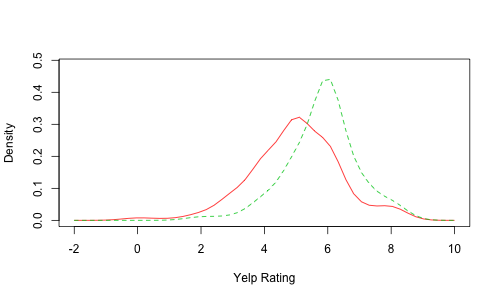
\includegraphics[width=0.5\textwidth]{Mission_ttest}
\end{figure}

Means are reported in converted Yelp rating, where 1 star is mapped to 0 and 5 stars is mapped to 8. There are no half-star or 0 star averages in the Yelp system. The result of our T-tests was that: Mexican food is significantly better in its respective district; Chinese food and Japanese food did not have significant differences. We decided to probe on beyond a binary predictor of rating.

\section{Experiment 2: Numerical Predictor}

Neighborhoods are geographical boundaries reflecting historical geographic makeup. We thought that a better signal than the neighborhood of a restaurant was the ethnic makeup of the restaurant's surroundings. Thus, we used the percent of the respective ethnicity (Asian, Black, White, Hispanic) in the 2010 Census as a predictor for the Yelp rating. The reason we used percent instead of quantity was that census tracts are approximated to 4000 people; thus, by using quantity, one would be approximating percentage. We fitted a linear model to each of Chinese, Japanese, Korean, Mexican, Thai and Vietnamese food.

\begin{center}
  \begin{tabular}{| l | c | c | c | c | c | r | }
    \hline
     & Itrcpt & co(p) & dof & p & RSE & Rsq \\ \hline \hline
    C & 4.64 & 0.01 & 382 & 0.97 & 1.154 & -0.002 \\ \hline
    J & 4.94 & -0.19 & 237 & 0.67 & 1.102 & -0.003 \\ \hline
    K & 4.62 & 1.29 & 49 & 0.125 & 0.868 & 0.028 \\ \hline
    M & 4.64 & 1.96 & 2e-16 & 265 & 1.122 & 0.126 \\ \hline
    T & 5.38 & -0.92 & 0.0176 & 127 & 0.858 & 0.036 \\ \hline
    V & 5.35 & -0.61 & 139 & 0.137 & 0.980 & 0.009 \\
    \hline
  \end{tabular}
\end{center}

\begin{figure}[h!]
  \caption{Mexican restaurant ratings versus Hispanic ethnic density}
  \centering
  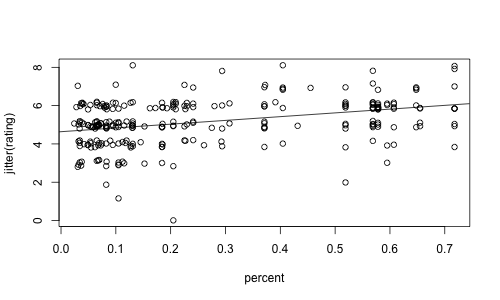
\includegraphics[width=0.5\textwidth]{mexican_regression}
\end{figure}

\begin{figure}[h!]
  \caption{Thai restaurant ratings versus Asian ethnic density}
  \centering
  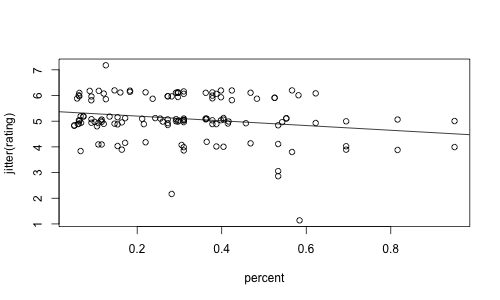
\includegraphics[width=0.5\textwidth]{thai_regression}
\end{figure}

The only food categories in which respective ethnic percentage was a meaningful predictor was Mexican food, at an R-Squared value of 0.126. This result set our expectations for how explanatory our variables would be. For Mexican food, the coefficient for percentage was 1.96, indicating that the difference between a 0\% Hispanic tract and 100\% hispanic tract is 1 Yelp star. A notable detail of the plot of rating vs. \% Hispanic was that there were virtually no low-rated restaurants in highly ethnic neighborhoods. The other significant regressions, such as Thai food, had a close-to-zero R-squared, and we interpreted this result as mostly due to having a lot of data.

Finally, we combined all businesses to determine if ethnic makeup was a significant predictor of ratings in general. (n = 1281)

\begin{center}
  \begin{tabular}{| l | c | c | c | r | }
    \hline
    Ethnicity & Coefficient & p & RSE & Rsq \\ \hline \hline
    Asian & -0.59 & 1.22e-5 & 1.119 & 0.014 \\ \hline
    Black & 0.44 & 0.222 & - & - \\ \hline
    Hispanic & 1.13 & 2.8e-9 & 1.112 & 0.026 \\ \hline
    White & 0.43 & 0.008 & 1.124 & 0.005 \\ \hline
  \end{tabular}
\end{center}

\begin{figure}[h!]
  \caption{Average restaurant rating versus white ethnic density}
  \centering
  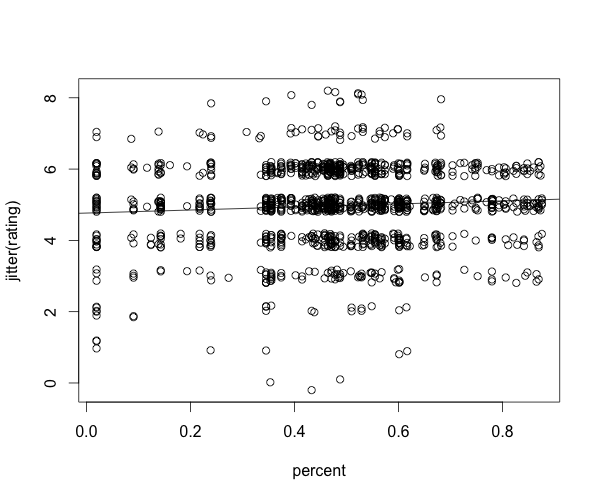
\includegraphics[width=0.5\textwidth]{whitepeople_presentation}
\end{figure}


Here, we also found significant predictors, but with close to zero R-squared values, these were not meaningful in explaining the variance of the data. Mutiple predictors and interactions were fitted with no significant effect. Based on these results, we felt that more detailed covariates may provide some more insight into ratings, beyond simple percentages.

\section{Additional Covariates: Density, Diversity, Price}

To construct the Density scalar for each census tract, we take the area (using shapely's area method) and divide it by the total population in that tract. This gives us a meaningful relative value for Density, although it has no unit meaning (since our polygons are defined in coordinates). We also did not reproject the geometry, since distortion is present equally among all the tracts.

To construct the Diversity scalar for each census tract, we referred to Sharma \cite{tindex}. The Theil Entropy index, used to measure the diversity of a Metropolitan Statistical Area, uses a Diversity index, D, for each census tract. This is calculated by sum(Pr(g) * ln (1 / Pr(g)) for all ethnic groups g. For our 4 ethnic groups, D varies from 0 to roughly 1.3, for a single ethnicity and an equal mix of all ethnicities, respectively.

Finally, we scraped Yelp manually to find the pricing information for each business, which varies from 1 (\$) to 4 (\$\$\$\$).

\section{Additional Hypotheses}
\begin{itemize}
\item Does density predict price or rating?
\item Does rating predict price?
\item Does diversity predict price or rating?
\item Of each ethnic cuisine, how dos rating vary with price?
\item Does anything predict ratings of vegetarian and vegan cuisine?
\end{itemize}
\section{Results}

First, we attempted to fit a linear model to rating using either price or density as predictors. We found neither is a significant predictor. Density was not a significant predictor of price, either. We did find that diversity was a significant predictor of both price and rating, but with a meaningless R-squared value.  A major flaw in the data preventing us from predicting price is that the output signal is only one of four values.

\begin{figure}[h!]
  \caption{Price versus ethnic density}
  \centering
  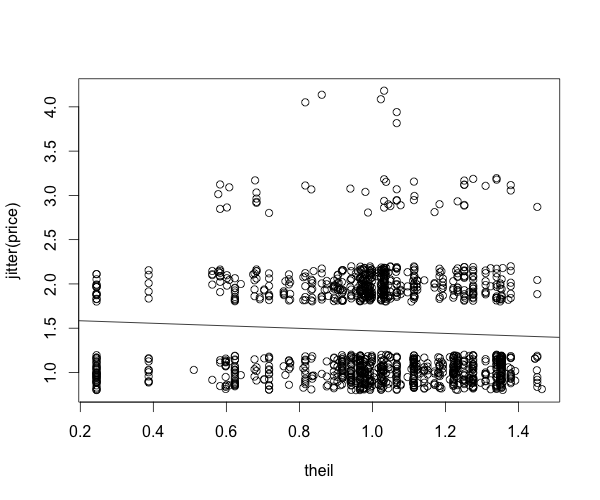
\includegraphics[width=0.5\textwidth]{diversity_price}
\end{figure}

We then attempted to find models for each ethnic cuisine. Finally, we found that density of ethnic populations are a significant predictor of Mexican food rating, but the R-squared (0.05) is low enough that when this integrated into a multiple predictor model, percent\% Hispanic still dominates. In conclusion, density as a predictor is less powerful than ethnic makeup; this reflects the neighborhood layout of San Francisco, since the densest neighborhoods are in Hispanic areas.

We cound not find any significant predictors for the combination of vegan and vegetarian foods. This was likely due to a sample size of only 70. One of the multiple-predictor models that we attempted was general rating predicted by both price and Diversity index. The fitted model gives significant predictors for both diversity and price, but again, neither are significant. In conclusion, our work found that Mexican food ratings are significantly predicted by dense ethnic neighborhoods, confirming our original hypothesis and supported that of our T-Tests. For other ethnicities, the data is just too noisy. For further work, we could easily expand this analysis to other cities.

\section{Data Product}

\begin{figure}[h!]
  \caption{Example map}
  \centering
  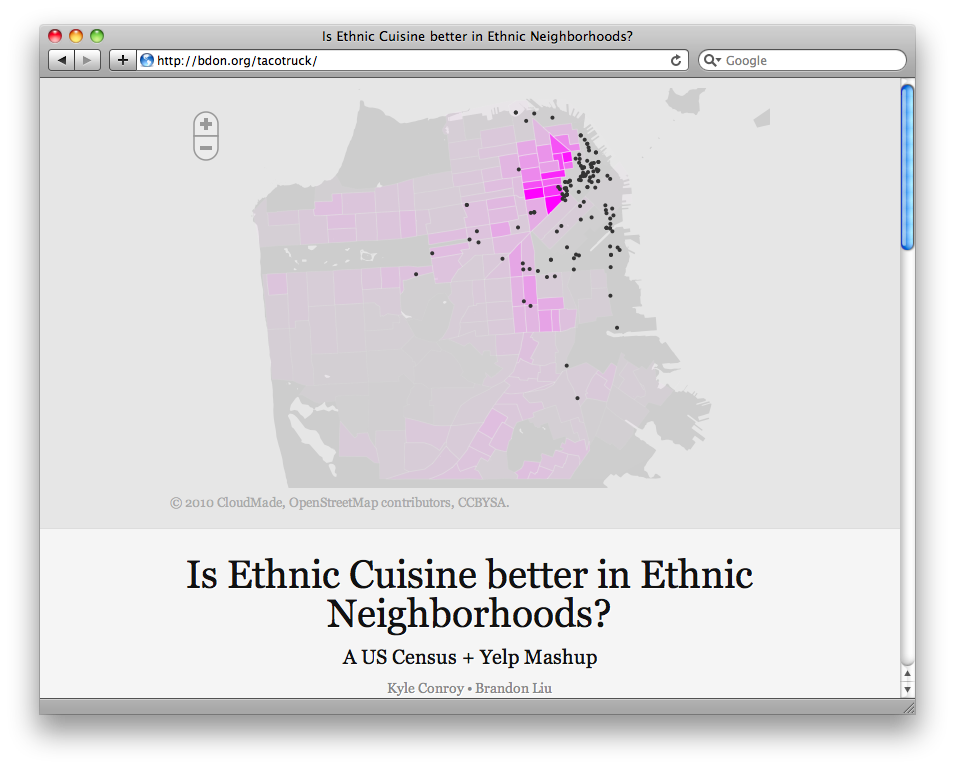
\includegraphics[width=0.5\textwidth]{webapp_screen}
\end{figure}

Our data product, available at http://bdon.org/tacotruck, shows thematic maps of San Francisco that users can browse. One such map shows Mexican restaurant ratings and corresponding ethnic population tracts on the same sequential color scale; since these are roughly correlated, the colors aid the viewer in picking out interesting points. Another map is the Diversity index plotted for all San Francisco census tracts.

\begin{thebibliography}{9}

\bibitem{yelpapi}
  Yelp Inc.,
  \emph{Examples of code using our API}.
  \url{https://github.com/Yelp/yelp-api}

\bibitem{pyshp}
  pyshp,
  \emph{Python Shapefile Library}.
  \url{http://code.google.com/p/pyshp/}

\bibitem{shapely}
  Shapely,
  \emph{GIS \& Python \& Invention}.
  \url{http://trac.gispython.org/lab/wiki/Shapely}

\bibitem{geos}
  GEOS Project,
  \emph{GEOS - Geometry Engine, Open Source}.
  \url{http://trac.osgeo.org/geos/}

\bibitem{foodtrucks}
  Department of Public Works - Bureau of Street-Use \& Mapping,
  \emph{Mobile Food Facility Permits}.
  \url{http://bsm.sfdpw.org/datasf/mobilefoodpermits.txt}

\bibitem{tindex}
  Madhuri Sharma,
  \emph{Spatial Integration and Neighborhood Diversity in Mid-Sized US MSAs, 1990-2000}.
  Graduate Research Associate,
  Center for Urban and Regional Analysis,

\bibitem{bcensus}
  Association of Bay Area Governments,
  \emph{Bay Area Census}.
  \url{http://www.bayareacensus.ca.gov/small/small.htm}

\bibitem{census}
  U.S. Census Bureau,
  \emph{Cartographic Boundary Files}.
  \url{http://www.census.gov/geo/www/cob/tr2000.html}

\end{thebibliography}

\end{document}
